\chapter{Implementation - Motion Planning}

This chapter covers the implementation methods on motion planning side of this project. Relevant code information can be found in User Guide Chapter.

\section{MoveIt! Interface and Planning Scene Setup} \label{motionplansetup}
As mentioned in Background Chapter, the motion planning part will utilize MoveIt!. The $moveit\_commander$ namespace is imported in order to use Python MoveIt! interface. This namespace contains a $RobotCommander$ class, a $MoveGroupComman$ $der$ class, and a $PlanningSceneInterface$ class.

A $RobotCommander$ object is firstly instantiated called $robot$. This object is the outer-level interface to the robot, which allow user to catch YuMi's names of joints, groups, and links and easy access to their properties.

To plan and execute motions on the YuMi, $MoveGroupCommander$ objects need to be instantiated as well. Each object should be one group of joints. In this case, the group can be $left\_arm$, $right\_arm$, and $both\_arms$. All of them are defined with the following settings.

\begin{table}[H]
\centering
\resizebox{\columnwidth}{!}{
\begin{tabular}{||c|c|c|c||}
\hline
Pose reference frame & Allow re-planning & Goal position tolerance & Goal orientation tolerance \\ \hline\hline
$yumi\_base\_link$ & False & 0.001 & 0.001 \\ \hline
\end{tabular}}
\caption{Settings of three $MoveGroupCommander$ objects: $left\_arm$, $right\_$ $arm$, and $both\_arms$}
\label{armsetup}
\end{table}

Moreover, a $PlanningSceneInterface$ object is instantiated, which is an interface to the world surrounding the robot. In this case, I defined the 3D position and 3D dimension of the workbench in front of YuMi, as shown in Figure \ref{scene}. By doing this, the workbench will be regarded as an obstacle to YuMi, so that the potential collisions between YuMi's arm(s) and the workbench can be avoided. However, the external cameras and other obstacles like workspace computer are not defined due to high measurement difficulty, by setting some safe poses for YuMi, the collisions can also be avoided. The details are discussed in Section \ref{safetyposescalculation}.

\begin{figure}[H]
\centering
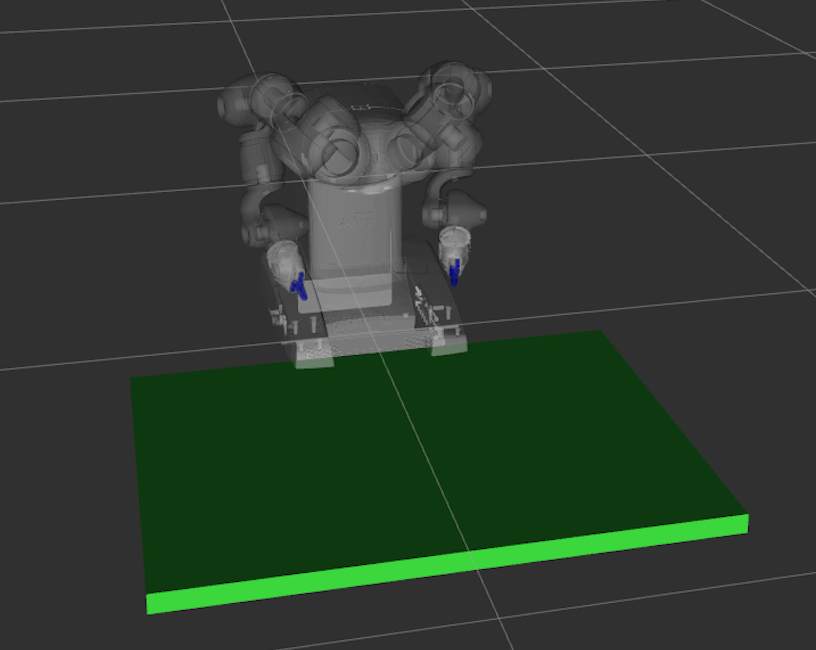
\includegraphics[width = 0.5\columnwidth]{Implementation/mp/planningscene.png}
\caption{The YuMi planning scene, where the workbench is defined as an obstacle.}
\label{scene}
\end{figure}

Finally, a $DisplayTrajectory$ publisher is created, which is utilized to publish trajectories for RViz to visualize:

\begin{minted}[frame=single, framesep=1.5mm, baselinestretch=1, fontsize=\footnotesize, linenos, breaklines]{python}
display_trajectory_publisher = rospy.Publisher('/move_group/display_planned_path', 	moveit_msgs.msg.DisplayTrajectory, queue_size=20)
\end{minted}


\section{Movement Control} \label{movementcontrol}
The opening and closing of YuMi' gripper(s) depend on the gripper effort value, which needs to be set between $-20$ to $20$. The gripper will open when the value is negative and close when it is positive. By publishing the effort value of specific gripper to its corresponding topic, $/yumi/gripper\_r\_effort\_cmd$ for right gripper, or $/yumi/gripper\_l\_effort\_cmd$ for left gripper, the gripper control function can be achieved. 

%(Whether the command is to open or close, the effort value will eventually set to 0 in order to relax the effort, which will not change the gripper state.)

As for YuMi's arm(s) control, it can be implemented in two ways: setting a joint goal or setting a pose goal.

\begin{itemize}
    \item \textbf{Joint Goal:} Each of YuMi's arm has 7 joints (shown in Figure \ref{yumijoint}). By setting them to specific value, every joint on the arm will rotate or bend accordingly to that configuration. The position of end-effector can be computed using forward kinematics.
    
    In this project, this approach is used to adjust YuMi's arm(s) to safe poses through the manipulation process, which will be introduced in Section \ref{safetyposescalculation}. In addition, shoelace adjustment after pulling ultilizes this method as well, which is introduced in Section \ref{shoelacegrabbing}.
\end{itemize}

\begin{figure}[H]
\centering
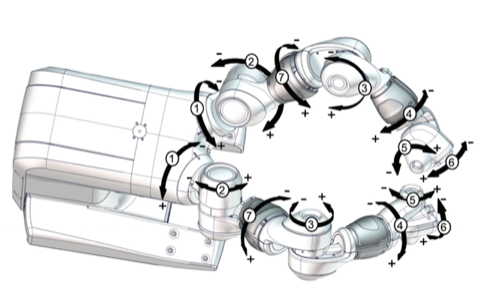
\includegraphics[width = 0.7\columnwidth]{Implementation/mp/yumijoints.png}
\caption{Joints of YuMi's arms \citep{Productspecification}}
\label{yumijoint}
\end{figure}

\begin{itemize}
    \item \textbf{Pose Goal:} The movement of a group can also be controlled by setting a pose goal for YuMi's end-effector(s) directly. The pose contains 3D position (x, y, z) and 3D orientation information (roll, pitch, yaw). The joint parameters that achieve this pose can be calculated via inverse kinematics. Notice that for the same pose goal, the joint parameters can be different.
    
    This method is used throughout the manipulation process including adjusting shoe pose, putting the lace through shoe hole, and grabbing the shoelace etc.
\end{itemize}

For single arm manipulation, letting the end-effector move to a pose goal can be achieved in two ways. Either using $compute\_cartesian\_path$ or $set\_pose\_target$ function. For a given pose goal, the former method will be tried first, and if it fails, the later one will be used. The $compute\_cartesian\_path$ function computes a Cartesian path that follows specified waypoints (6D poses). The maximum resulting step size between the end-effector configurations of consecutive points in the result trajectory is predefined, which is 0.005 that provides a resolution of $5mm$. Collision and kinematic will be checked and if these constraints cannot be met, the function will return a fraction of the path achieved between $0$ and $1$. If successful, fraction will equal to $1$.

\begin{minted}[frame=single, framesep=1.5mm, baselinestretch=1, fontsize=\footnotesize, linenos, breaklines]{python}
(plan, fraction) = cur_arm.compute_cartesian_path(waypoints, 0.005, 0.0, True)
\end{minted}

While the $set\_pose\_target$ function can be used for both single and dual arm motion planning. Its inputs are simply the target 6D pose and the name of corresponding end-effector. Following is the dual arm plan and move function for this project utilizing $set\_pose\_target$. 

\begin{minted}[frame=single, framesep=1.5mm, baselinestretch=1, fontsize=\footnotesize, linenos, breaklines]{python}
def plan_and_move_dual(target_l, target_r):
    group_both.set_pose_target(target_l, "yumi_link_7_l")
    group_both.set_pose_target(target_r, "yumi_link_7_r")
    plan = group_both.plan()
    group_both.go(wait=True)
    rospy.sleep(3)
\end{minted}



\section{Safe Poses Calculation} \label{safetyposescalculation}

\begin{figure}[H]
\centering
\subfigure[Cal pose]{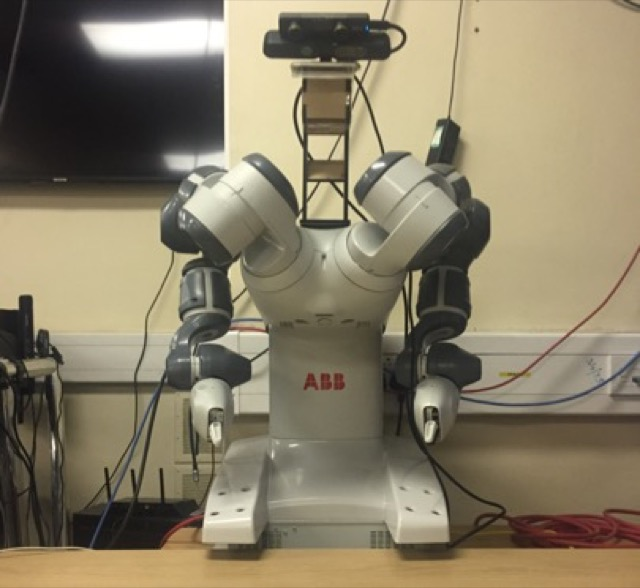
\includegraphics[width = 0.32\columnwidth]{Implementation/mp/calpose.jpg}}
\subfigure[Home pose]{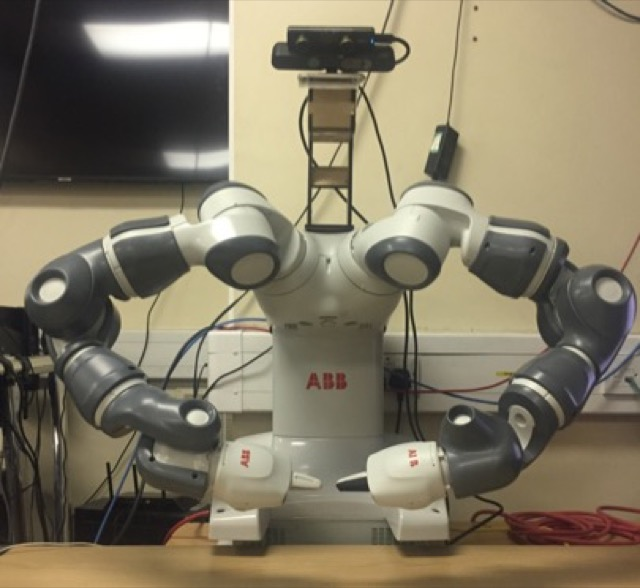
\includegraphics[width = 0.32\columnwidth]{Implementation/mp/homepose.jpg}}
\subfigure[Initial pose]{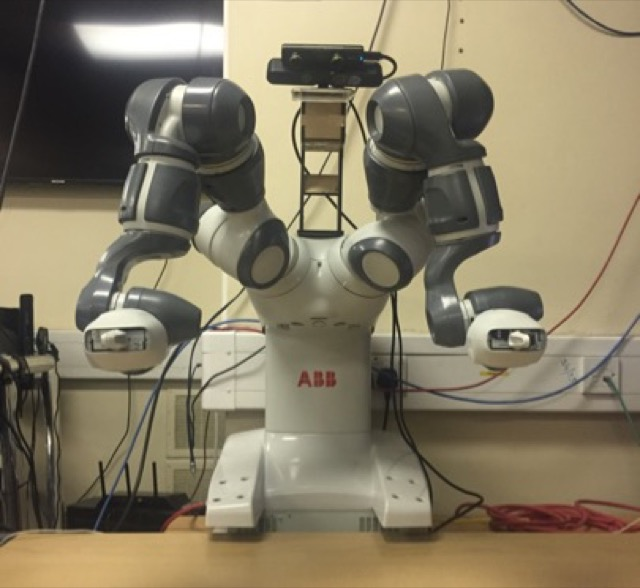
\includegraphics[width = 0.32\columnwidth]{Implementation/mp/initialpose.jpg}}
\caption{Safe poses of YuMi}
\label{safeposition}
\end{figure}

Figure \ref{safeposition} shows three pre-defined safe poses of YuMi: cal pose, home pose and initial pose. For each manipulation, YuMi will start with cal pose, then move to either home or initial pose before performing the tasks. Once it finishes the job, it will move back to home or initial pose before finally returning to cal pose. By doing so, YuMi's arm(s) will always move in front of and under the cameras, which prevents potential collisions with the cameras and the workspace computer.

The 14 joint parameters ($safeJointPositionR$ and $safeJointPositionL$) of these safe poses are measured by using $get\_current\_joint\_values$ function, after moving YuMi's arms to
these desired poses in Rviz. For each safe pose, the joint goals can the be set accordingly. Following is the code example to plan and move both arms to a safe pose.

\begin{minted}[frame=single, framesep=1.5mm, baselinestretch=1, fontsize=\footnotesize, linenos, breaklines]{python}
elif (arm == BOTH):
    group_both.set_joint_value_target(safeJointPositionL + safeJointPositionR)
    group_both.plan()
    group_both.go(wait=True)
\end{minted}

\section{Shoe Pose Adjustment} \label{adj}
As mentioned in Section \ref{shoeadjust}, if the shoe is vertically placed, then its orientation needs to be adjusted. Recall the idea illustrated in Figure \ref{adjustmentidea}, in which YuMi will use both arms. In Section \ref{shoeadjust}, the real-world locations of $adr$, $adrr$, $adl$, $adll$ have already been computed and published to $TF$.
Here, their locations referenced to YuMi frame $yumi\_base\_link$ can be calculated using $lookupTransform$ function. Following is the example applied on location $adr$, where $rospy.Time(0)$ provides the latest available transform.

\begin{minted}[frame=single, framesep=1.5mm, baselinestretch=1, fontsize=\footnotesize, linenos, breaklines]{python}
(trans_adr,_) = self._tfsub.lookupTransform('/yumi_base_link', '/adr', rospy.Time(0))
\end{minted}

The output $trans\_adr$ is the 3D location (x, y, z) of a waypoint. However, the z location and 3D rotation of $adr$ will not be used because they can be pre-defined before the adjustment process. The z coordinate is set as $0.1$ and the rotation is $[-\frac{\pi}{4}, \pi, \pi]$ for left gripper and $[\frac{\pi}{4}, \pi, \pi]$ for right gripper in order to provide the best Angle of application. Figure \ref{realadjust} shows the real adjustment process. The detailed waypoints for this process can be found in Table \ref{adjustwaypoints}.

\begin{figure}[H]
\centering
\subfigure[Move to pre-adjustment]{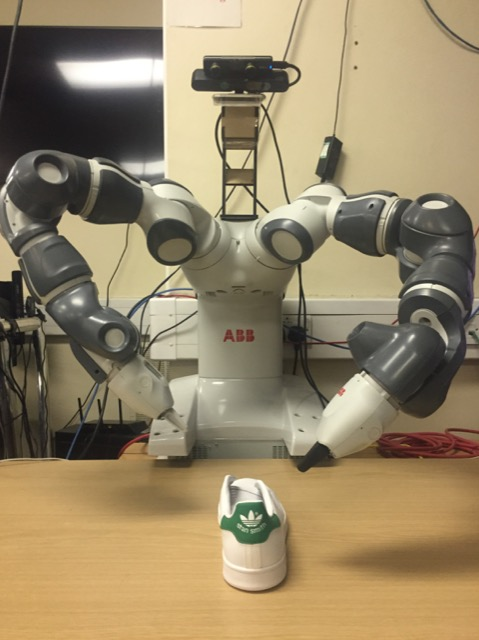
\includegraphics[width = 0.19\columnwidth]{Implementation/mp/adj2.jpg}}
\subfigure[Move down to $adr$ and $adl$]{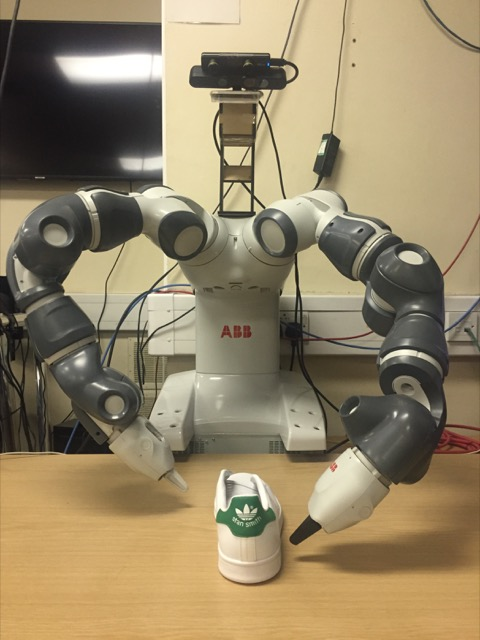
\includegraphics[width = 0.19\columnwidth]{Implementation/mp/adj3.jpg}}
\subfigure[Move to $adrr$ and $adll$]{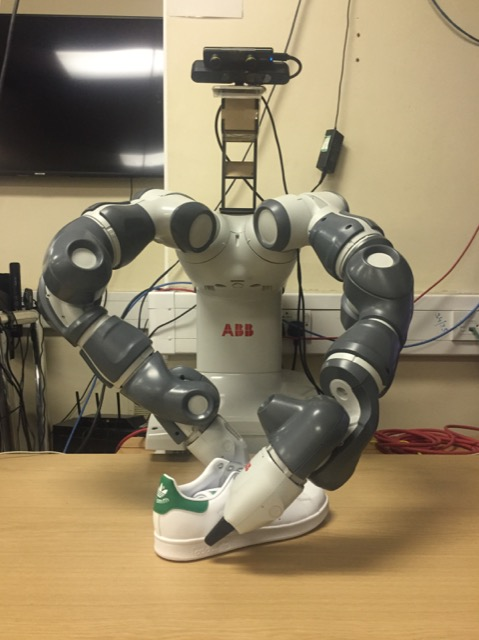
\includegraphics[width = 0.19\columnwidth]{Implementation/mp/adj4.jpg}}
\subfigure[Move back to $adr$ and $adl$]{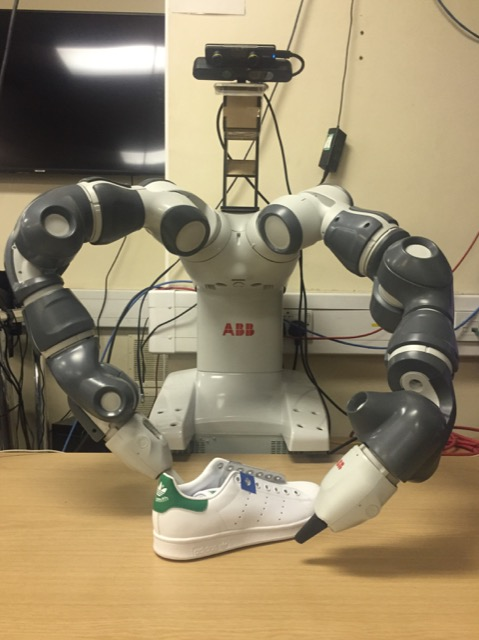
\includegraphics[width = 0.19\columnwidth]{Implementation/mp/adj5.jpg}}
\subfigure[Move up to post-adjustment]{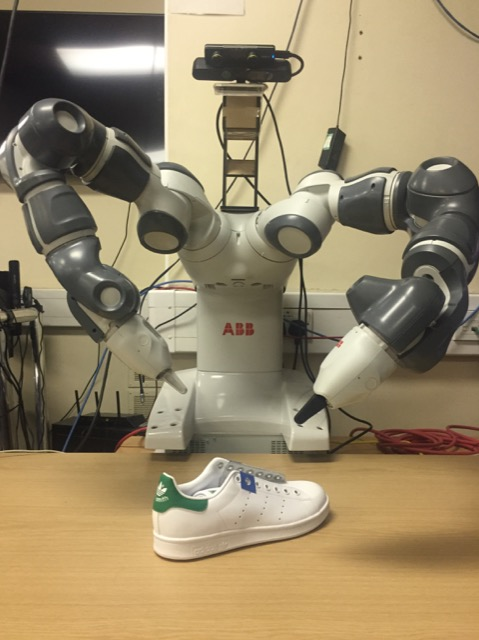
\includegraphics[width = 0.19\columnwidth]{Implementation/mp/adj6.jpg}}
\caption{The example motion process for shoe pose adjustment. YuMi starts from cal pose then moves to home pose before going to (a), and returns to home and finally moves back to cal pose after (e).}
\label{realadjust}
\end{figure}

Figure \ref{preposeadjust} shows the detected shoe hole before and after adjustment, the later gives a much more accurate results. Figure \ref{shoeposerange} illustrates the possible orientation range of the shoe hole after adjustment. The hole will face towards the camera, either to hole's top-left or top-right.

\begin{figure}[H]
\centering
\subfigure[Detected shoe hole before and after adjustment for example illustrated in Figure \ref{realadjust}]{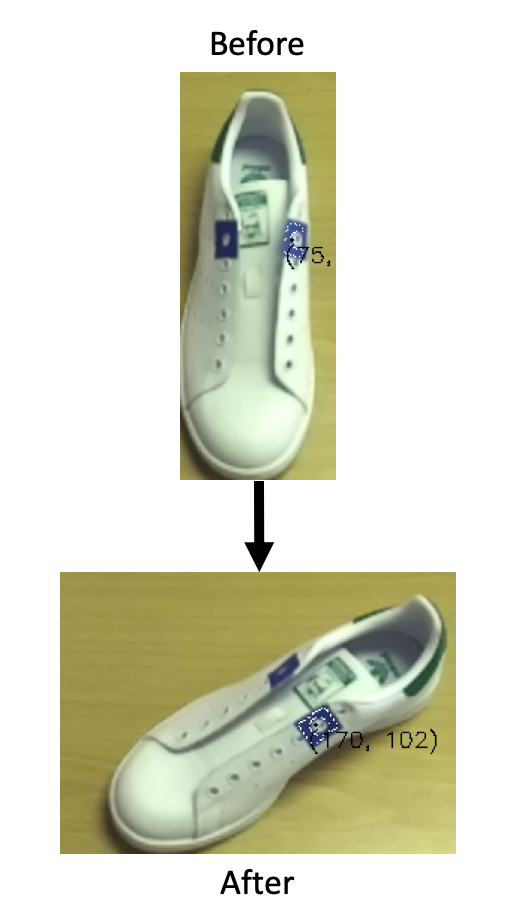
\includegraphics[height = 7.5cm, keepaspectratio]{Implementation/mp/shoebaadj.png} \label{preposeadjust}}
\subfigure[Ideal orientation range of shoe hole after adjustment. The shoe hole should face either to it's top-left or top-right.]{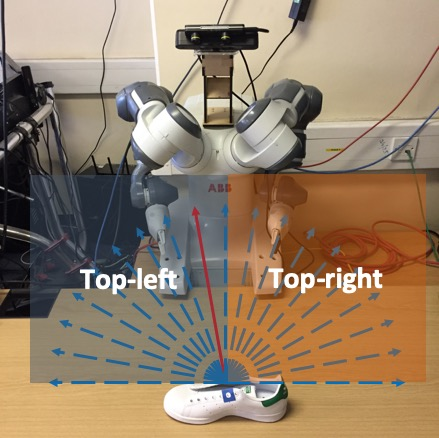
\includegraphics[height = 7.5cm, keepaspectratio]{Implementation/mp/toplefttopright.jpg} \label{shoeposerange}}
\caption{The adjustment results and ideal shoe orientation range}
\end{figure}


\section{Robot Gripper Approaching Pose} \label{approachposegripper}
When the orientation of the shoe is ideal, YuMi will start to put the shoe lace into the hole by using the computed $shoe\_hole$ and $pre\_put$ information. Same as the method used in previous section, these two locations are firstly transformed to $yumi\_base\_link$ frame, which gives the coordinates of $(x, y, z)$ and $(xn, yn, zn)$.

\begin{figure}[H]
\centering
\subfigure[Orange solid line indicates the ideal gripper orientation]{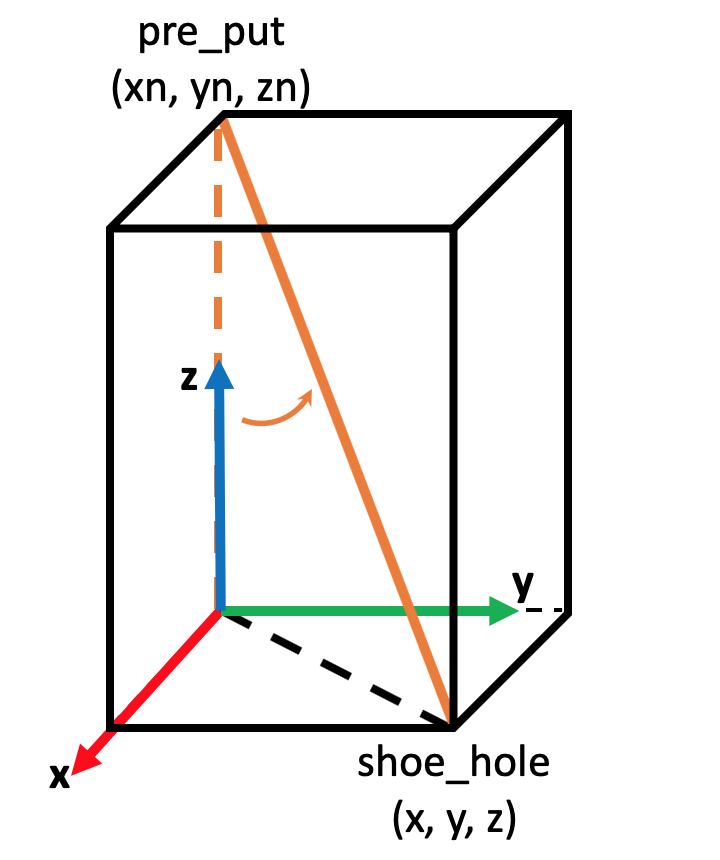
\includegraphics[width = 0.31\columnwidth]{Implementation/mp/ap1.png} \label{gripperap}}
\subfigure[Calculation of roll rotation a]{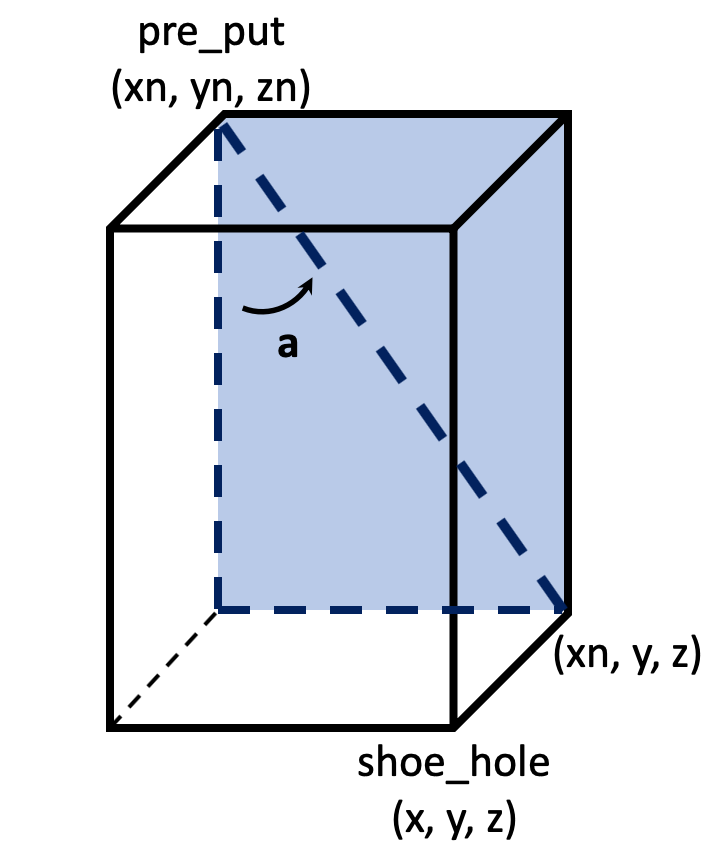
\includegraphics[width = 0.31\columnwidth]{Implementation/mp/ap2.png} \label{roll}}
\subfigure[Calculation of pitch rotation b]{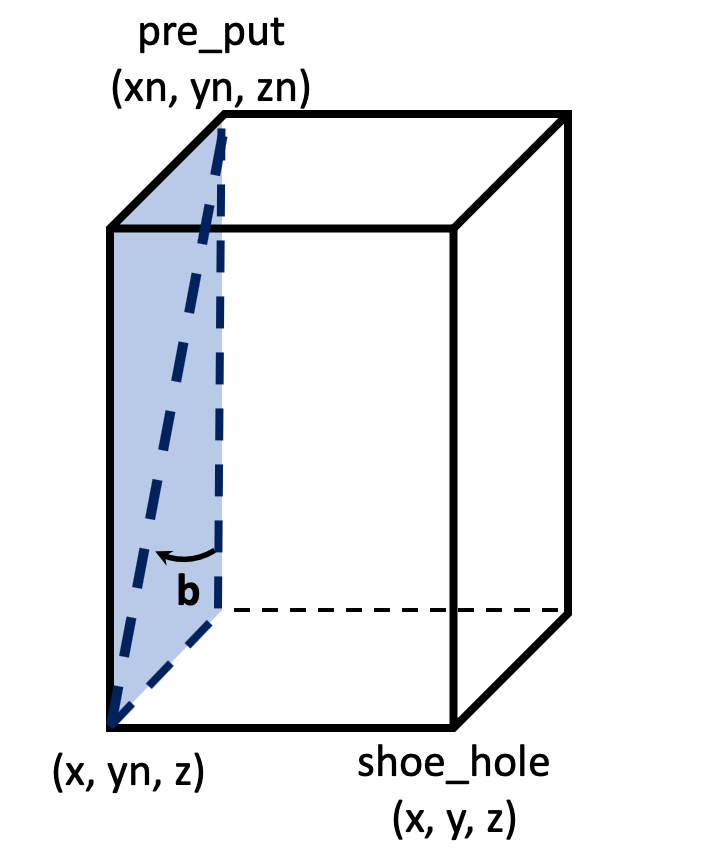
\includegraphics[width = 0.31\columnwidth]{Implementation/mp/ap3.png} \label{pitch}}
\caption{Top-left case: gripper approaching orientation computation}
\end{figure}

Recalling the project requirements, before YuMi starts to manipulate the shoelace, one of its grippers is holding it. In this project, the beginning orientation of the shoelace is considered to be the same as that of the gripper, as mentioned in Section \ref{3DOrientationofShoeHole}. Therefore, to put it into the shoe hole, the orientation (roll, pitch, yaw) of gripper\slash shoelace needs to be aligned with the normal vector of the plane surrounding with the shoe hole. As shown in Figure \ref{gripperap}, for the situation when the shoe hole is orienting to its top-left, this direction is represented as the solid orange line. 

When gripper is facing the ground (the vertical orange dash line in Figure \ref{gripperap}), it has 3D rotation $(0, \pi, \pi)$. Therefore, the alignment can be split into two steps: roll alignment (Figure \ref{roll}) and pitch alignment (Figure \ref{pitch}). There is no need to consider yaw alignment for this step, because the shoelace insertion will not be affected no matter what angle it is. Thus, yaw will be kept as $\pi$.

\begin{equation}
a = \arctan \frac{y - yn}{zn - z}
\label{rollcalculation}
\end{equation}

\begin{equation}
b = \arctan \frac{x - xn}{zn - z}
\label{pitchcalculation}
\end{equation}

By using Equation \ref{rollcalculation} and \ref{pitchcalculation}, the roll and pitch angles can be computed. Because the shoe is assumed in an ideal pose (orienting to its top-left or top-right), $a$ will be in the interval $[-\frac{\pi}{2}, \frac{\pi}{2}]$ and $b$ always lies in range $[0, \frac{\pi}{2}]$. Recall that the beginning configuration of gripper pitch angle is $\pi$, therefore the finally 3D orientation of YuMi gripper should be $(a, b + \pi, \pi)$. 

So far, the preliminary pre-insertion pose is $[xn, yn, zn, a, b + \pi, \pi]$ and the preliminary insertion pose is $[x, y, z, a, b + \pi, \pi]$. However, these poses are not accurate enough for this precision task, whose offsets need to be further adjusted.

\section{Offset Adjustment and Shoelace Insertion} \label{offsetadjustment}
When letting YuMi's gripper move to a specific 3D location detected by ZED Mini camera with default orientation $(0, \pi, \pi)$ (facing the ground), the system needs to add $-0.021$ offset on the x-axis ($x\_offset$), $0.009$ offset on the y-axis ($y\_offset$), and $0.145$ offset on the z-axis ($z\_error$) to achieve relatively precise movement. However, the offset adjustment becomes complicate when the gripper varies its orientation.

\begin{figure}[H]
\centering
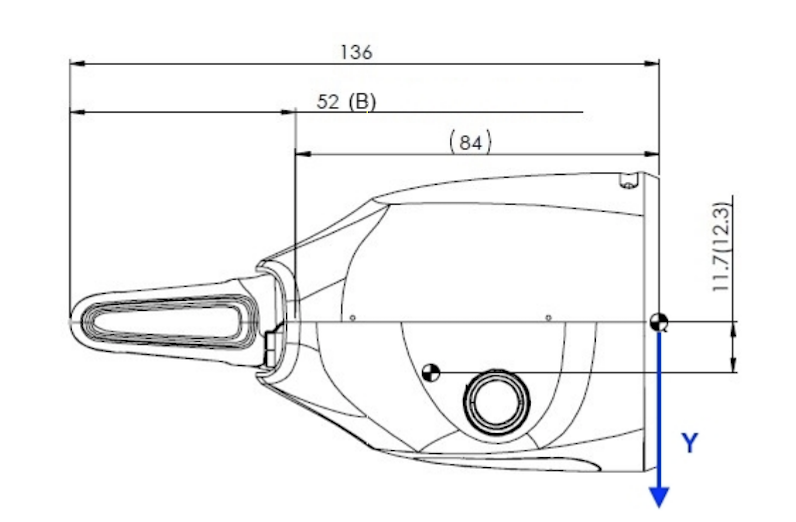
\includegraphics[width = 0.8\columnwidth]{Implementation/mp/gripperoffset.png}
\caption{YuMi's gripper design, adopted from \citep{Productspecification}. The distance between the endpoint of the gripper and the end-effector is 136 mm.}
\label{gripperoffset}
\end{figure}

When planning and moving YuMi's arm(s) by setting pose goals, it is all about the pose of the end-effector. Figure \ref{gripperoffset} shows the design of the YuMi' gripper. It can be discovered that the distance between the endpoint of the gripper and the end-effector is $136mm$. Therefore the offset on z-axis contains $0.136$ gripper offset and $0.009$ system offset ($z\_offset$).

\begin{figure}[H]
\centering
\subfigure[X-axis gripper offset due to pitch rotation $b$]{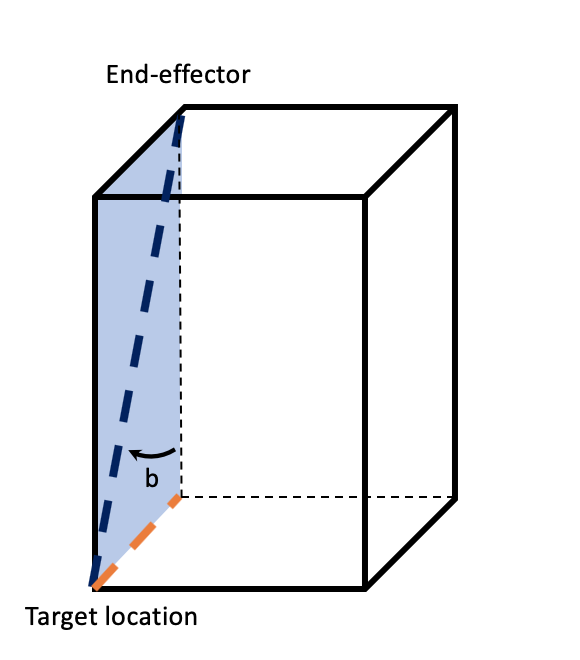
\includegraphics[width = 0.32\columnwidth]{Implementation/mp/off3.png}\label{offsetx}}
\subfigure[Y-axis gripper offset due to roll rotation $a$]{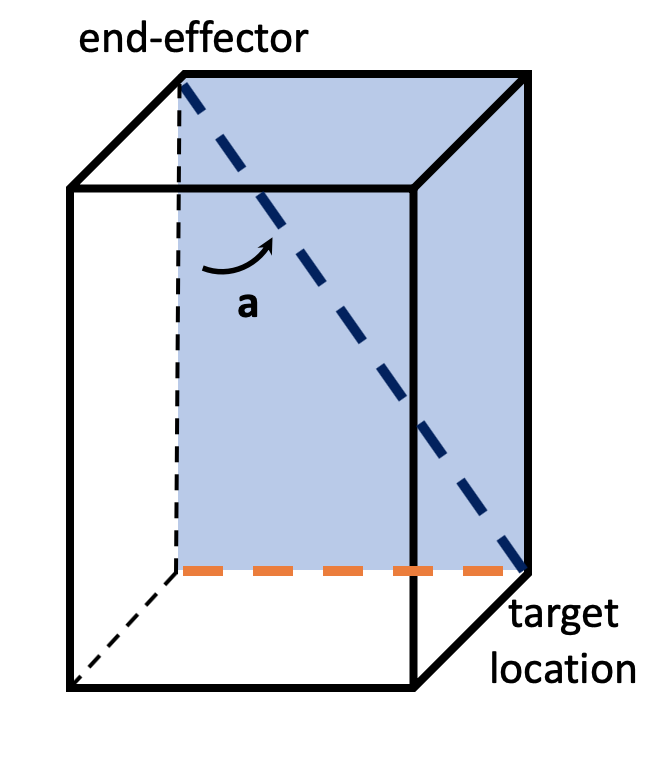
\includegraphics[width = 0.32\columnwidth]{Implementation/mp/off2.png}\label{offsety}}
\subfigure[Z-axis gripper offset due to both roll and pitch rotation]{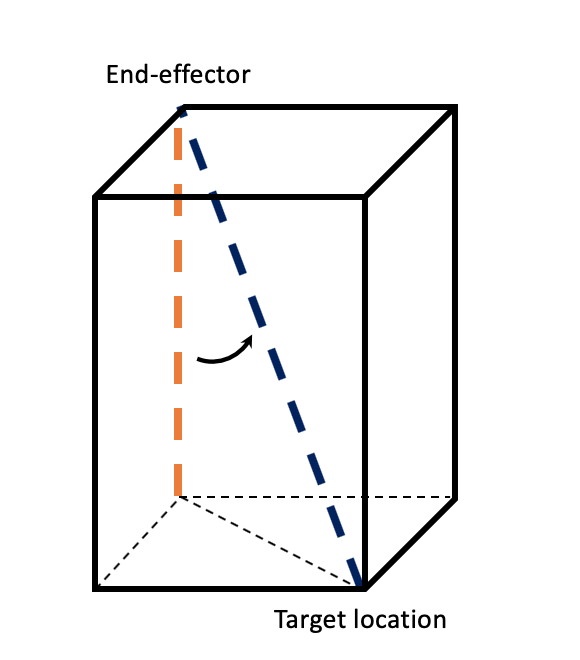
\includegraphics[width = 0.32\columnwidth]{Implementation/mp/off1.png}\label{offsetz}}
\caption{Top-left case: the gripper offset adjustment, where the dark blue dash lines represent gripper offset 0.136mm, the orange dash lines are the corresponding offsets introduced by it.}
\label{offset}
\end{figure}

%In Figure \ref{offset}, the dark blue dash lines represent gripper offset 0.136, the orange dash lines are the corresponding offsets introduced by it.

Once the gripper performs rotations, this gripper offset will affect the $(x, y, z)$ location the gripper endpoint reaches. For Figure \ref{offsetx}, if the gripper has a pitch angle of $b$ and the endpoint of the gripper needs to reach the "target location", the end-effector only should be at location "end-effector". The same issue occurs for roll rotation as well (see Figure \ref{offsety}). Furthermore, z-axis offset is affected by both of them. To reach the same target location with rotations, the end-effector needs to move down more than that in default orientation. This is because the influence of gripper offset on the z-axis is diluted by the other two axes.

\begin{equation}
xoff = x\_offset - gripper\_offset*sin(b)
\label{xoff}
\end{equation}

\begin{equation}
yoff = y\_offset - gripper\_offset*sin(a)
\label{yoff}
\end{equation}

\begin{equation}
zoff = gripper\_offset*cos(a)*cos(b) + z\_offset
\label{zoff}
\end{equation}

Equation \ref{xoff}, \ref{yoff}, and \ref{zoff} provide the approaches to calculate the final offsets of the three axes. The final pose goals for putting the shoelace into a hole are illustrated in Equation \ref{Preput} and \ref{Insertion}. Figure \ref{putexample} shows an example of the shoelace insertion process.

\begin{equation}
pre\_insertion = post\_insertion = [xn + xoff, yn + yoff, zn + zoff, a, b + \pi, \pi]
\label{Preput}
\end{equation} 

\begin{equation}
insertion\_pose = [x + xoff, y + yoff, z + zoff, a, b + \pi, \pi]
\label{Insertion}
\end{equation} 

\begin{figure}[H]
\centering
\subfigure[Move to initial pose, shoelace is attached manually]{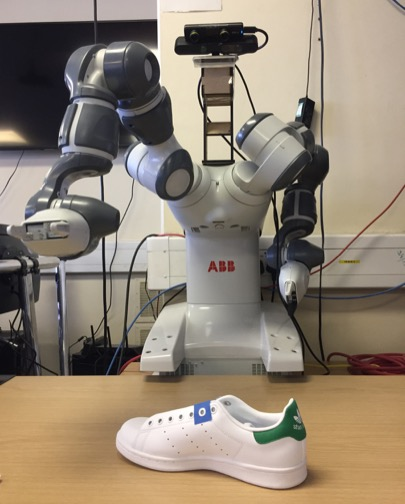
\includegraphics[width = 0.19\columnwidth]{Implementation/mp/1put.jpg}}
\subfigure[Move to $pre\_$ $insertion$ pose]{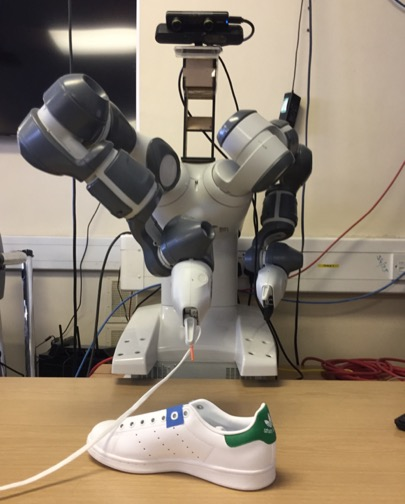
\includegraphics[width = 0.19\columnwidth]{Implementation/mp/2put.jpg}}
\subfigure[Move to $insert$ $ion\_pose$ and ope\-n the gripper]{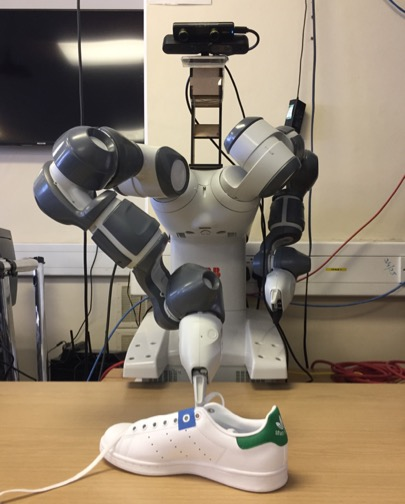
\includegraphics[width = 0.19\columnwidth]{Implementation/mp/3put.jpg}}
\subfigure[Move back to $post\_insertion$]{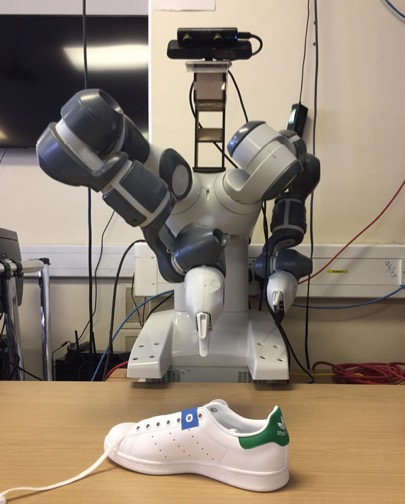
\includegraphics[width = 0.19\columnwidth]{Implementation/mp/4put.jpg}}
\subfigure[Move back to initial pose]{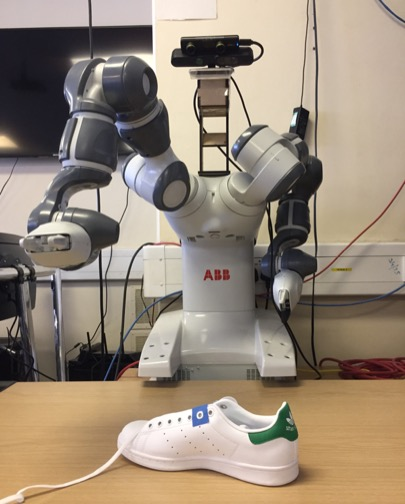
\includegraphics[width = 0.19\columnwidth]{Implementation/mp/5put.jpg}}
\caption{The example motion procedure for inserting shoelace into a target hole. YuMi starts from cal pose then move to (a), and goes back to cal pose after finishing the task (e).}
\label{putexample}
\end{figure}

\section{Shoelace Grabbing} \label{shoelacegrabbing}
After the shoelace being passed through the hole, YuMi should locate this shoelace and pull it out to complete this single hole. Since the endpoint of a shoelace is straight, the orientation of the shoelace is considered to be aligned with this direction. Therefore, the approximately location of shoelace can be computed using the normal vector calculated in Section \ref{3DOrientationofShoeHole}. Given the normal vector $n = Ai + Bj + Ck$, the grab location is set as $(0.05*A, 0.05*B, 0.05*C)$ referenced to $shoe\_hole$, where $0.05$ is used to define the distance between them. Figure \ref{pick} shows the related frames in Rviz, where $pre\_put$, $shoe\_hole$, and $pick$ are on the same normal vector. Here, the $pick$ location will be transformed to $yumi\_base\_link$ frame as well, which gives the coordinate $(xp, yp, zp)$.

\begin{figure}[H]
\centering
\subfigure[Real-world shoe placement. The shoe is in a good pose, thus it will not be adjusted.]{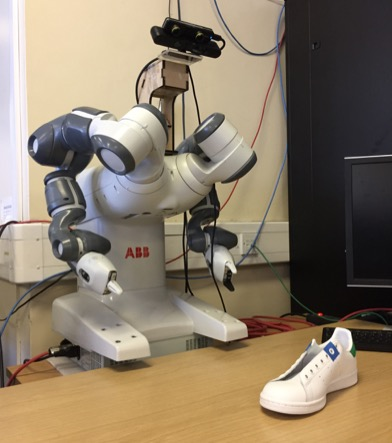
\includegraphics[height=6cm,keepaspectratio]{Implementation/cv/3dposw.jpg}}
\subfigure[The frame relationships in Rviz. The $pre\_put$, $shoe\_hole$ and $pick$ locations are on the same line.]{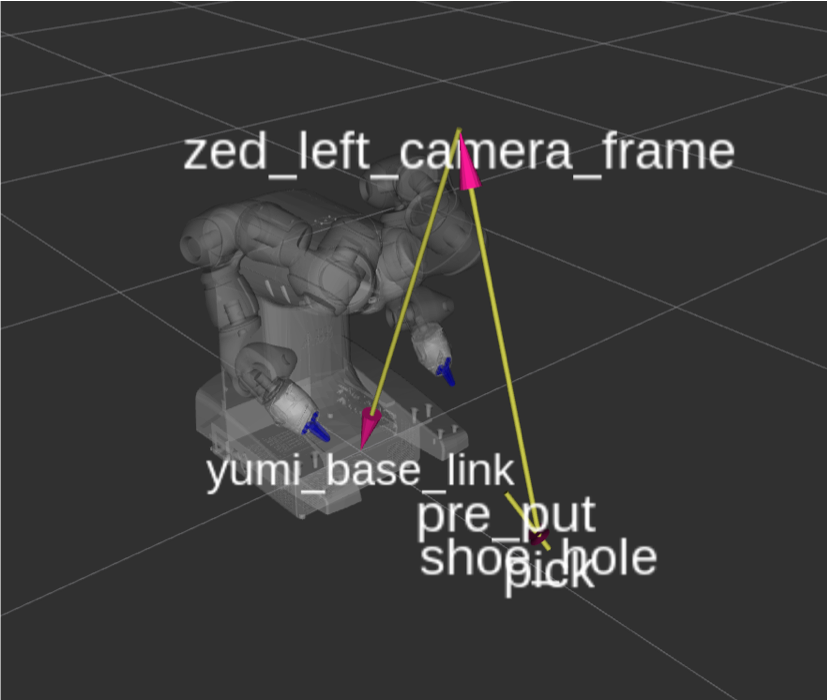
\includegraphics[height=6cm,keepaspectratio]{Implementation/cv/pickrviz.png}\label{pick}}
\caption{Example of shoe lace pose estimation using ZED Mini.}
\end{figure}

%The idea to solve this problem is shown in Figure \ref{lacegrab}, where the orange arrow represents the direction in which the shoelace is inserted into the hole.

\begin{figure}[H]
\centering
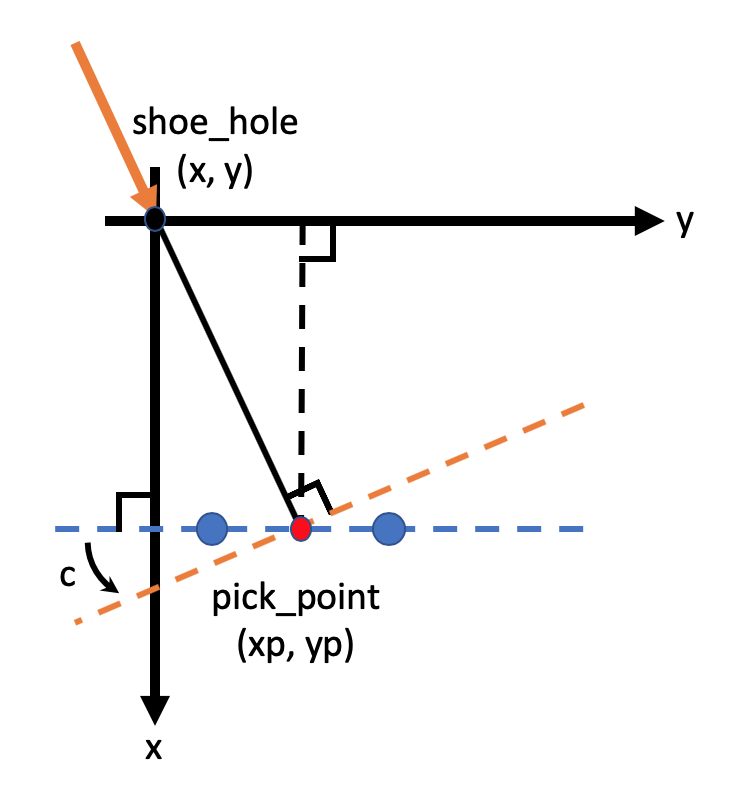
\includegraphics[width = 0.5\columnwidth]{Implementation/mp/lacegrab.png}
\caption{Top-left case: 2D Top view that contains the shoe hole position, ideal shoelace pickup position, etc. The orange arrow represents the direction (normal vector) in which the shoelace is inserted into the hole.}
\label{lacegrab}
\end{figure}

The method to solve this shoelace grabbing problem is shown in Figure \ref{lacegrab}. When YuMi's gripper is perpendicular to the inserting direction (the orange arrow), YuMi will have the highest probability to complete this task. In other words, the two fingers of the gripper should be at the two orange points respectively, which aligns with orange dash line. In this case, when the gripper closes, the shoelace can be grabbed. 

The parameter that controls the rotation of the gripper on the z-axis is yaw. When YuMi's fingers are at two blue points in Figure \ref{lacegrab}, the yaw rotation is $\frac{\pi}{2}$. Thus, there is an angle $c$ needs to be added, which can be calculated according to Equation \ref{yawcalculation}.

\begin{equation}
c = \arctan \frac{yp - y}{xp - x}
\label{yawcalculation}
\end{equation}

Considering both top-left and top-right cases, the available range of $c$ is $[-\frac{\pi}{2}, \frac{\pi}{2}]$. When this condition is satisfied, the final grabbing pose can be written as Equation \ref{grabpose}. Notice that, here, the offset for 3D location is different form that of $pre\_insertion$ and $insertion\_pose$. This is because this time the gripper does not perform any roll and pitch rotations from its default orientation.

\begin{equation}
grabbing\_pose = [xp + x\_offset, yp + y\_offset, zp + z\_error, 0, \pi, c + \frac{\pi}{2} - 0.1]
\label{grabpose}
\end{equation}

In addition, $-0.1$ is added to yaw rotation. This angle adjustment prevents gripper from getting stuck on the sides of the shoe. As for $pre\_grabbing$ pose and $post\_grabbing$ pose, they are the same as the $grabbing\_pose$ except theirs $z$ parameters are $0.1m$ higher, which allow the gripper to approach the shoelace more safely.

\begin{figure}
\centering
\subfigure[Move to home pose]{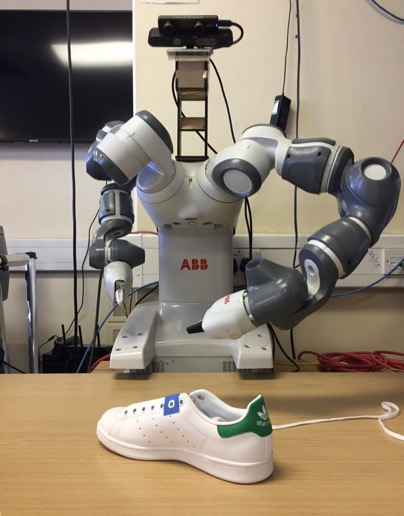
\includegraphics[width = 0.19\columnwidth]{Implementation/mp/1pull.jpg}}
\subfigure[Move to $pre\_$ $grabbing$ and open the gripper]{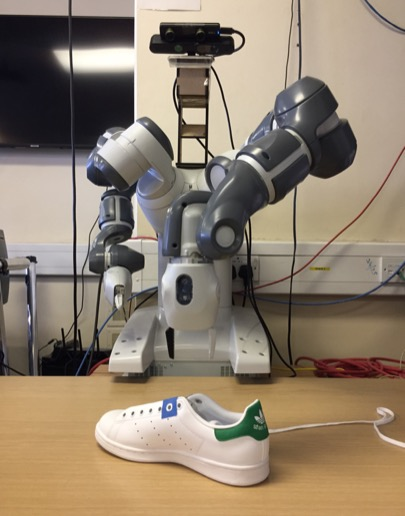
\includegraphics[width = 0.19\columnwidth]{Implementation/mp/2pull.jpg}}
\subfigure[Move to $grab$ $bing\_pose$ and clo\-se the gripper]{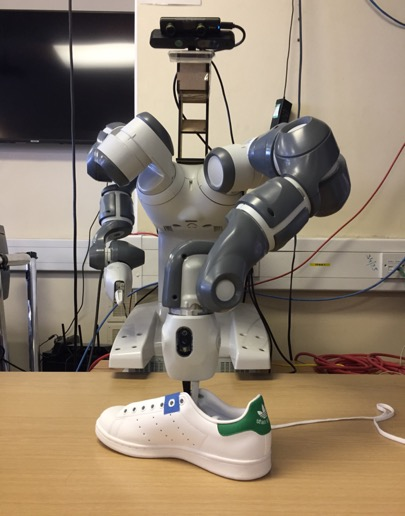
\includegraphics[width = 0.19\columnwidth]{Implementation/mp/3pull.jpg}}
\subfigure[Move back to $post\_grabbing$]{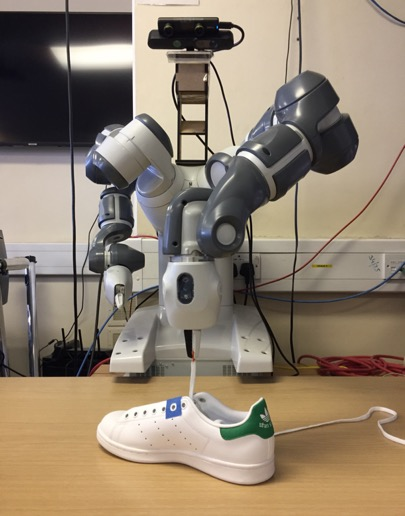
\includegraphics[width = 0.19\columnwidth]{Implementation/mp/4pull.jpg}}
\subfigure[Move upwards to pull the shoelace out]{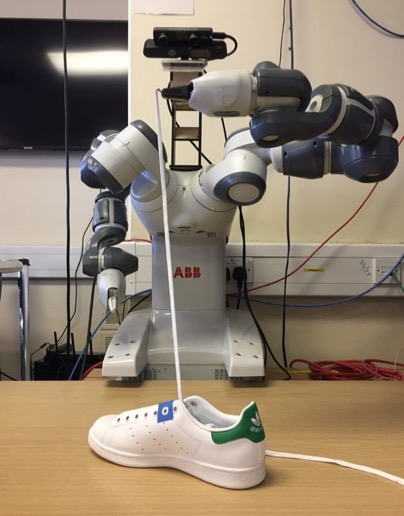
\includegraphics[width = 0.19\columnwidth]{Implementation/mp/5pull.jpg}}
\subfigure[Move down to let the lace hang naturally]{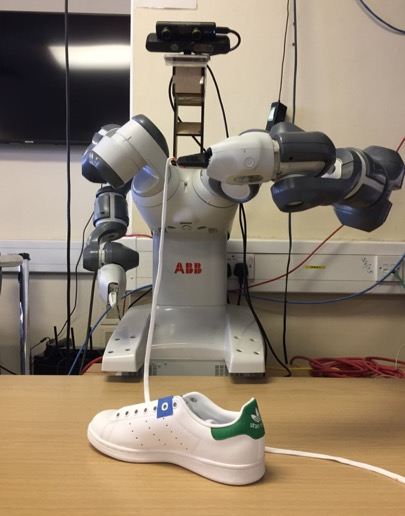
\includegraphics[width = 0.19\columnwidth]{Implementation/mp/6pull.jpg}}
\subfigure[Move right gripper below left gripper]{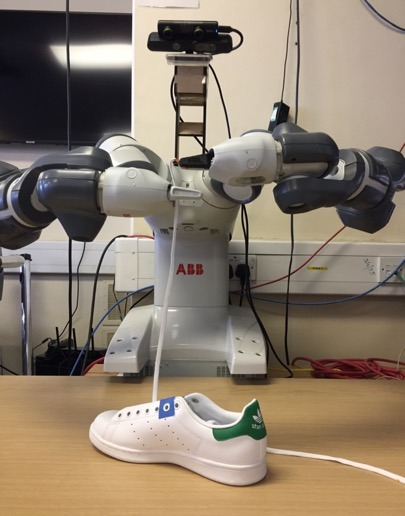
\includegraphics[width = 0.19\columnwidth]{Implementation/mp/7pull.jpg}}
\subfigure[Close the right gripper]{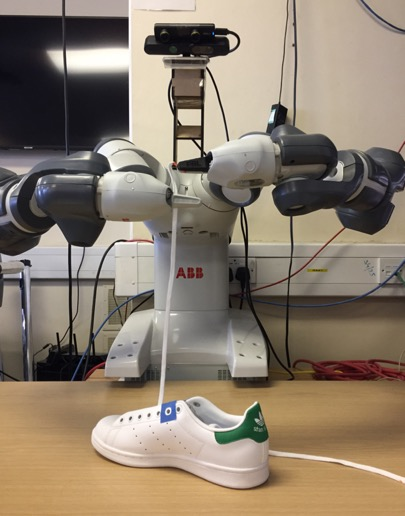
\includegraphics[width = 0.19\columnwidth]{Implementation/mp/8pull.jpg}}
\subfigure[Move right gr\-ip\-per forwards and open left gripper]{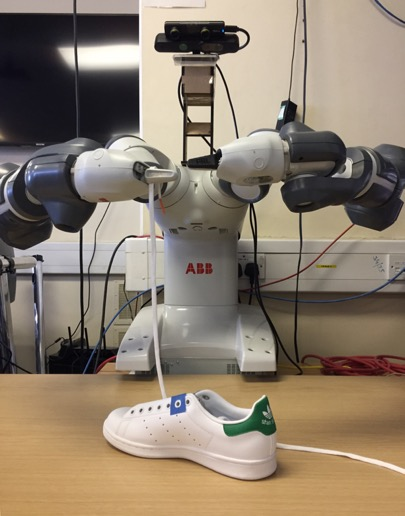
\includegraphics[width = 0.19\columnwidth]{Implementation/mp/9pull.jpg}}
\subfigure[Move left arm back to home pose]{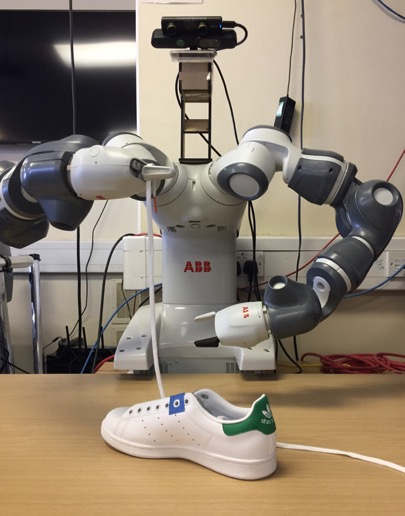
\includegraphics[width = 0.19\columnwidth]{Implementation/mp/10pull.jpg}}
\caption{The example motion process of grabbing and pulling shoelace out. YuMi starts from cal pose before moving to (a). The grabbing process finishes at (d). From (e) to (j) is about shoelace pulling and adjusting. YuMi moves back to cal pose after (j).}
\label{pickexample}
\end{figure}

Figure \ref{pickexample} displays the shoelace grabbing and pulling process, where YuMi firstly uses its left arm. It starts from cal pose, then moves to (a) home pose before executing, and moves back to $post\_grabbing$ pose (d) after grabbing. The series of motions after (e) is for shoelace adjustment, which aims to let another gripper grasp the lower part of the shoelace, so that its colored head can be seen by the camera. To achieve this task, YuMi will firstly pull the shoelace out in (e), then move downwards to let the it hang naturally. After that the right gripper will move below the left gripper for clamping. To prevent the head from falling behind gripper which blocks the camera's view, in (i), the right arm will then move slightly away from the camera before the left gripper opening. Finally, the left arm will return to home pose (j) and go back to cal pose. 

All of the motions from (e) to (j) are planned by setting joint goals. Therefore, the posture of both arms is fixed every time. Figure \ref{3dlace} displays the camera view at stage (j).

\begin{figure}[H]
\centering
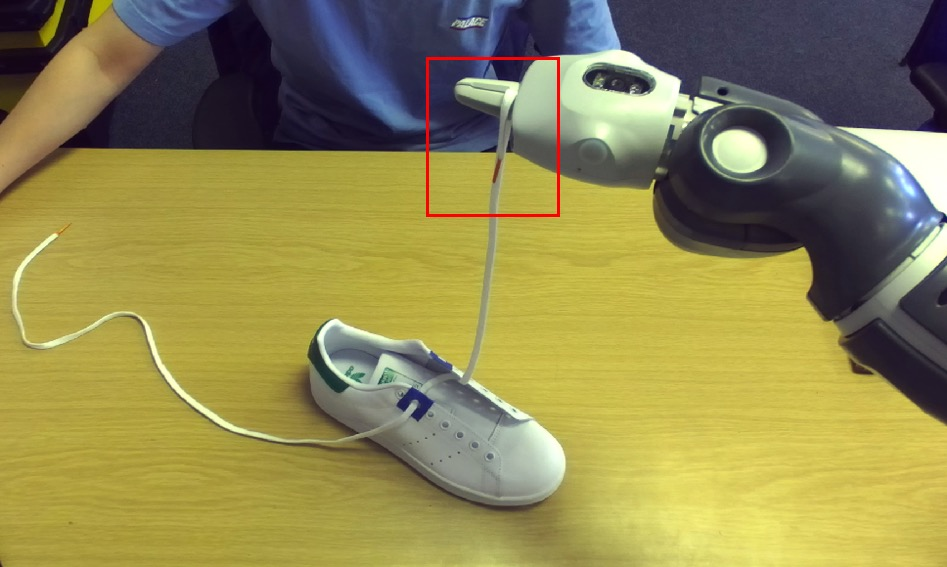
\includegraphics[width = 0.6\columnwidth]{Implementation/mp/3dlace.jpg}
\caption{The camera view at stage (j) of Figure \ref{pickexample}. The shoelace will always be in the red bounding box.}
\label{3dlace}
\end{figure}

Since the arm pose is static each time, the colored head of shoelace will always appear in the red bounding box in Figure \ref{3dlace}. Using the same approach as discussed in Section \ref{3dlocationestimation} and \ref{3DOrientationofShoeHole}, the the 3D location and 3D orientation of the shoelace can be computed. By employing similar method introduced in Section \ref{approachposegripper}, the left gripper is able to align its direction with the colored head and re-clamp. After the orientation of the shoe being adjusted based on the algorithm in Section \ref{shoeadjust} and \ref{adj} using one single arm, YuMi will be ready to perform insertion for the next hole. The whole shoe can be eventually completed according to this workflow.